
\chapter{【李斯的月夜和雨夜】}
\begin{wrapfigure}{r}{0.3\textwidth}
\centering
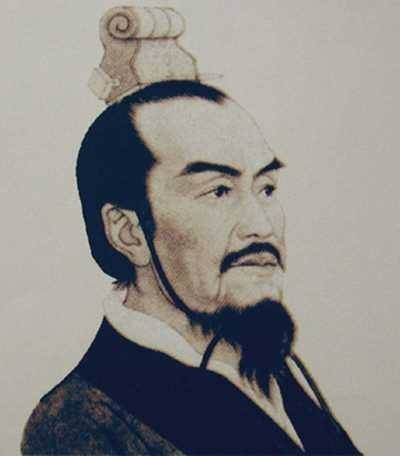
\includegraphics[width=0.3\textwidth]{pics/p003.jpg}
\vspace{-25pt}
\caption{李斯}
%\label{test}
\end{wrapfigure}

文/李碧華
\footnote{摘自《讀者》雜誌2018年9月號[言論1]與【讀者雜誌讀書會】臉書社團,圖:摘自網路}

26歲的李斯,是楚國一個看守糧倉的小文書。
糧囤附近有草葦圍住的糞坑。
李斯如廁時,見到枯瘦瑟縮又沾了糞的小耗子,
他想:人生如鼠啊,不在倉就在廁。
他不禁長歎:「一輩子有無出息,全看為自己找一個什麼位置。」

在一個月夜,他想,該換一種活法了。

清早,他匆匆離開家鄉、親人、沒前途的把老鼠腰斬的守倉員職位 $\cdots$ 這一走,
終其一生沒有再回去。他高升了。

很多年以後,他像當日殺鼠一樣,被判五刑加腰斬—劓刖、割舌、剁肢、笞殺同時執行之際便腰斬,最後慢慢碎屍。
一家老小、三族親戚、賓客門生 $\cdots$ 不分男女,一律斬首。
七八個劊子手斧起刀落,也是一直忙到傍晚,雨夜。雨整整下了一個月。

以上是錢寧作品{\Kai《秦相李斯》}中生死興衰的始末。

在辭典裡,再慘烈也不過占了幾句:「秦朝丞相,定郡縣制,開中國地方制度新局面。
為趙高誣陷謀反,腰斬於咸陽。」而腰斬,在中國古代酷刑中,也不過其中一項而已。

每一個人,當要過另一種生活時,必然也有另一種結局在等他。
這是當時的貨倉管理員上廁所時所料想不到的。
而斬殺他的指鹿為馬的趙高,亦逃不了「夷三族」的下場。

歷史便是這樣了。

